%\documentclass{acm_proc_article-sp}

\documentclass{article}

\usepackage{mathpartir}
\usepackage{turnstile}
\usepackage{amssymb}
\usepackage{amsmath}
\usepackage{stmaryrd}
\usepackage{graphicx}
\usepackage{epsfig}
\usepackage{subfigure}
\usepackage{listings}
\usepackage{natbib}
\usepackage{verbatim}
\usepackage[utf8]{inputenc}
\usepackage[T1]{fontenc} 
\usepackage[hyphens]{url}
\lstset{language=ml}
\lstset{commentstyle=\textit}
\lstset{mathescape=true}
\lstset{backgroundcolor=,rulecolor=}
\lstset{frame=single}
\lstset{breaklines=true}
\lstset{basicstyle=\ttfamily}

\begin{document}

\title{Presenting: the Casanova language \\the next generation of game programming}

\begin{comment}
\numberofauthors{4}
\author{
Giuseppe Maggiore \and Enrico Steffinlongo \and Renzo Orsini \and Michele Bugliesi \\
       \affaddr{Universit�  Ca' Foscari Venezia}\\
       \affaddr{Dipartimento di Scienze Ambientali,}\\
       \affaddr{Informatica e Statistica}\\
       \email{\{maggiore,orsini,bugliesi,esteffin\}@dais.unive.it}
}
\end{comment}

\date{}

\maketitle

\begin{abstract}
Games are extremely complex pieces of software which give life to animated virtual worlds. Games require complex algorithms, large worlds filled with many intelligent entities and high-quality graphics, and it all must run in real time.

Building general, high-performance frameworks capable of representing any virtual world has, until now, proven to be an elusive task; existing solutions either sacrifice performance (X3D browsers) or generality (game engines).

In this paper we present a new language, called Casanova, that aims at incorporating the knowledge that game engines represent with libraries or framework inside a language. The language is built around the idea of a single game state which contains not only its shape but also a series of rules that define how the state updates itself at every tick of the game engine. Rules are well suited for describing the declarative portions of the game update, but in order to keep the language expressive and easy to use we introduce behaviors, a system of imperative coroutines that run combined with the rules.

Rules and behaviors are coupled with powerful optimization techniques such as parallel execution, memory recycling and query optimization (for set processing) which greatly improve the performance of a game without requiring careful manual implementation of complex optimization algorithms.
\end{abstract}

\begin{comment}
\category{D.1.1}{Programming Techniques}{Applicative (Functional) Programming} 
\category{D.2.2}{Soft\-ware Engineering}{Software Libraries}[Design Tools and Techniques]
\category{D.2.13}{Soft\-ware Engineering}{Reusable Software}[Domain engineering, Reusable libraries, Reuse models]
\category{D.3.3}{Programming Languages}{Language Constructs and Features}
\category{D.3.4}{Pro\-gramming Languages}{Processors}[Optimization, Run-time environments]
\category{H.5.1}{Information Systems}{Information Interfaces and Presentation}[Multimedia Information Systems]

\terms{Games,Performance,Languages}

\keywords{games, compilation}
\end{comment}


\section{Introduction}
\label{sec:intro}
%%%%%%%%%%%%%%%%%%%%%%%%%%%%%%%%%%%%%%%%%%%%%%%%%%%%%%%%%%
% intro.tex
%%%%%%%%%%%%%%%%%%%%%%%%%%%%%%%%%%%%%%%%%%%%%%%%%%%%%%%%%%


\begin{figure}
\begin{center}
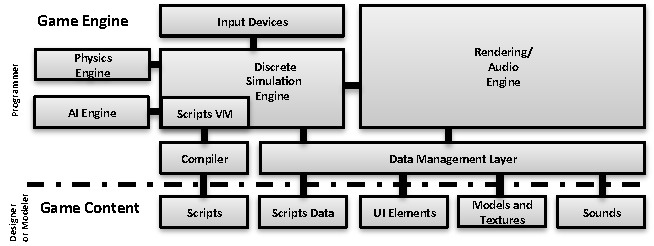
\includegraphics[scale=0.8]{engine_architecture.pdf}
\end{center}
\label{fig:data_driven_games}
\caption{Data-driven engine architecture, from \cite{SGL}}
\end{figure}

Virtual reality browsers face big challenges centered on performance and complexity. Performance is needed because the framerate at which the virtual world is rendered and animated must be high enough to give the user a feeling of smoothness. The scene must be rendered at least at 30 frames per seconds, but higher framerates (e.g. 60 frames per second) are perceived by the user as more pleasant.

Both the visual and logical complexities of a virtual world are very important. Visual richness gives the user the impression of a more realistic and detailed world, with many beautifully rendered objects, while logical complexity permits articulated responses that give the user the feeling of being part of a realistic world with its own set of rules and internal laws.

One of the most important tasks for developers of interactive worlds is to find the right trade-off between these sometimes conflicting requirements. Increasing performance requires a mixture of compromise (reducing the size of the world or ``dumbing down'' its responses) and time-consuming low-level optimization. We believe that automated optimization of interactive applications is a fundamental frontier if we wish to enable developers to build richer worlds without exponentially increasing costs.

Modern 3D browsers and engines are based on a data-driven architecture as shown in Figure \ref{fig:data_driven_games}, taken from \cite{SGL}.

In a data-driven engine the engine contains only general knowledge about virtual worlds, but nothing specific about the peculiar features of a specific virtual world. The specific virtual world will be loaded from the game content in the form of configuration files and scripts. A data-driven engine loads from files two main datasets:

\begin{itemize}
\addtolength{\itemsep}{-0.5\baselineskip}
\item a \textbf{scene}, the set of entities that populate the virtual world
\item \textbf{scripts}, the set of (possibly complex) behaviors that animate the scene entities
\end{itemize}

The scene is composed by a heterogeneous set of entities, each of a different kind. Entities may be virtual characters, trees, 2d or 3d models; entities may also be purely logical and invisible entities such as timers, triggers and proximity sensors.

Scripts give depth to a scene by implementing complex interrelationships between entities. Scripting can be done at three different levels of increasing complexity and expressive power:

\begin{itemize}
\addtolength{\itemsep}{-0.5\baselineskip}
\item \textit{routing} is a simple transmission of values from one entity to another
\item more complex scripts can perform data conversions when moving information between entities
\item even more advanced scripts can create, remove or modify entities of a scene
\end{itemize}

The usual implementation of an engine (see \cite{GAME_OO_HIERARCHY}) features an object-oriented architecture of classes. At the root of this architecture is a class that represents the most generic entity, and from which all other entities are derived. The engine maintains a list of these generic entities, which are all updated and handled through a set of virtual functions. This architecture is a source of often underestimated overhead. Dynamic dispatching is not too costly for a few calls, but when we have many entities, the cost of invoking various virtual functions many times for each frame can become very high. Sometimes the cost of the dynamic dispatching architecture may become higher than the cost of the actual operations being dispatched.

Scripts usually access the scene dynamically. This means that a script must look for the right entities with a mixture of lookups by name and unsafe casts. For example, consider how a Java script may access the \texttt{time} field of a \texttt{myClock} node of type \texttt{timer}:

\begin{lstlisting}
\addtolength{\itemsep}{-0.5\baselineskip}
X3DNode myClock = 
 mainScene.getNamedNode("myClock");
SFTime time = 
  (SFTime) myClock.getField("time");
\end{lstlisting}

This style is unsafe, since \texttt{myClock} may not exist or it may have the wrong type, and it also incurs in significant overhead.

In this paper we will focus exclusively on the X3D language, since it is a recognized standard and it offers a good benchmark to test virtual worlds where we can specify our scene and its various scripts. In the paper we show how we have tackled the problem of increasing performance in X3D browsers while also making scripts safe. We have used a simple compilation technique that removes many unnecessary dynamically dispatched invocations; this technique also allows us to introduce safety for scripts that access the state, so that they do not need to perform unsafe dynamic lookups when searching for specific nodes. To the best of our knowledge, this is the first approach that experiments with compiling X3D scripts and scenes in order to achieve greater performance and safe scripts. None of the previous approaches we are aware of focuses on compilation of X3D as a means to achieve both higher performance (by reducing overhead) and safety (by introducing compile-time checks). Higher performance through compilation includes a long list of research work such as \cite{OPT1,OPT2,OPT3} which has shown that compilation can yield better runtime performance by reducing dynamic overhead and improving other properties of the generated code. Similarly, introducing safety in dynamic languages such as scripting systems has been studied in general in the context of generating typed programs from untyped scripts in \cite{SAFESCRIPTS1}, and the problem of statically typing information which is generally untyped has also been explored in the Haskell community in \cite{SAFESCRIPTS2} among many others.

In Section \ref{sec:solution_workflow} we discuss the general architecture of our system. In Section \ref{sec:compiling_scene} we show how our technique generates the code and the type definitions that represent a scene. In Section \ref{sec:case_study} we show an example of a compiled scene and its routes. In Section \ref{sec:benchmarks} we report some benchmarks that show speed increasing when rendering a sample scene with just nodes and routes by applying our technique. Finally, in Section \ref{sec:compiling_scripts} we discuss how we represent scripts that externally access the scene.

 

\section{Existing game engines}
\label{sec:game_engines}
%%%%%%%%%%%%%%%%%%%%%%%%%%%%%%%%%%%%%%%%%%%%%%%%
% GAME ENGINES
%%%%%%%%%%%%%%%%%%%%%%%%%%%%%%%%%%%%%%%%%%%%%%%%

Games and their complex requirements.

\subsection{Related Work}
- Data driven games
- Entity hierarchy
- Components
- Against OO in games
- Handmade optimizations
- Nightmare of concurrency
- SGL
- Dungeon Siege
- The X3D/VRML Way (general but no performance)

\subsection{A different approach}

Game engines as world interpreters:
- data driven = game data + scripts = an actual, complex, interpreter

Rather than interpret, we build a language to compile the world rather than interpret it (less overhead).

A general framework for games:
- rules
- behaviors
Rules and behaviors in existing genres:
- arcade
- puzzle
- racing
- rts
- fps
- rpg

We define a language around the idea of rules and behaviors, but with optimization firmly in mind.
Also, with a language we can:
- do syntactic abstraction, reducing boilerplate code (recycling memory efficiently, repetitive algorithmic optimizations, traversing the game state for updating, etc.)
- encouraging a declarative style of programming which can yield to an increase in productivity by writing less code at a higher leve of abstraction, that is with lower maintenance costs
- to simplify the approach to game programming and encouraging the emergence of a single idiom by providing only aspects essential to this domain, rather than using a very general purpose programming language with lots of paradigms (all somewhat acceptable but ultimately inadequate to the domain)
- to enforce certain important properties at the semantics level, in order to allow the automation of important constructs such as complex cross-module optimizations

Our language does not take care about graphics. Casanova is a language capable of building the simulation module which can then be linked with another program capable of performing the rendering. 

\section{The Casanova language}
\label{sec:casanova}
%%%%%%%%%%%%%%%%%%%%%%%%%%%%%%%%%%%%%%%%
% THE CASANOVA LANGUAGE
%%%%%%%%%%%%%%%%%%%%%%%%%%%%%%%%%%%%%%%%

In this section we present the Casanova language; for a more detailed treatment, see \cite{CASANOVA_TR}. Casanova is inspired to the ML family of languages.

\subsection{Design Goals}
We have designed the Casanova language with multiple goals in mind. First of all, Casanova games must be easy and intuitive to describe. For this reason we have used a mix of declarative and procedural programming. For expressing rules, declarative programming is simple, allows the developer to focus on what he wants to achieve rather than how, and there is a wealth of powerful optimization techniques for declarative operations on sequences of values coming from the field of databases \cite{QUERY_OPT}. The declarative portions of a game are all executed in parallel, and can take advantage of multi-core CPUs.

Procedural programming, in particular coroutines \cite{COROUTINES}, are used to describe computations that take place during many ticks of the game engine. Imperative coroutines are used to express the behaviors of a game. These behaviors are executed sequentially and with no optimizations, since they can access any portion of the state both for reading and writing, and they may perform any kind of operation.


\subsection{A brief introduction to Casanova}
Casanova is a programming language designed aroung a set of core principles aimed at aiding game development. Here we describe the language ``at a glance'', by listing its features designed to simplify repetitive, complex or error prone game coding activities: \textit{(i)} Casanova integrates the game loop and time as first-class constructs. The game loop and time management are almost always an important part of game development libraries, for example see \cite{XNA}; \textit{(ii)} it performs a series of optimizations that are usually found hand-coded in virtually all game engines \cite{GAME_OPT}, such as logical optimization of queries on lists and spatial partitioning/use of indices to speed up quadratic queries such as collision detection (for example: \texttt{colliders(self) = [other | other <- Others, collides(self,other)]}; \textit{(iii)} it guarantees that updates to the game state during one tick are consistent, that is the state is never partially updated thanks to a (high-performance) transactional system; \textit{(iv)} it offers a scripting system that integrates seamlessly with the update loop.

We have designed Casanova with the aim of adding more features such as: \textit{(i)} automated generation of all the rendering code; \textit{(ii)} automated generation of all the networking code; \textit{(iii)} automated generation of all or parts of an AI system.

Of course the language can also serve as a general purpose language. Any application that requires performing computations and visualization on a complex set of data which evolves over time according to a set of fixed rules might benefit from using Casanova. In the future we may investigate other possible uses of the language in this direction.
As a final remark,it must be noted that Casanova sometimes constrains the developer; for example, at most one rule may be associated with any given field of the game state and rules are always applied at every tick of the simulation. Since developers may find this set of restrictions too tight we have included a scripting system which can also act as a ``wildcard'' in this  regard, that is scripts have essentially no limitations in expressivity (scripts are a general purpose programming language with coroutines) and for this reason they can be used to express anything that the rule system cannot, albeit renouncing various useful features such as automated optimization.

\subsection{Syntax, Semantics and Types}
The details of the Casanova language syntax, semantics and type system are defined in \cite{CASANOVA_TR}. In this subsection we give a general overview of the most salient aspects of the language.

A Casanova program is divided into three parts: \textit{(i)} the state definition, \textit{(ii)} the initial state and \textit{(iii)} the main behavior.

The state definition contains the type definitions of the game state and game entities, together with the rules the various fields are subjected to. Rules may be nested, that is a field may contain a rule of type \texttt{Rule T}, where \texttt{T} contains a value of type \texttt{Rule V}. This is quite common, and we will seen an instance of this in the example below (in the \texttt{Introductory Example} subsection).

Entities and the state may be defined in terms of the usual type constructors found in a functional language: records, tuples and discriminated unions. Also, we can define values of type: table (for sequences), variable (for mutable cells), rule (for updateable fields) and reference (for read-only pointers).

The initial state defines the starting value of the various game entities.

The main behavior is an imperative process which runs for the entire duration of the game. A behavior may spawn (\texttt{run}) other behaviors, suspend itself for one or more ticks (\texttt{yield} or \texttt{wait}) or wait for another behavior to complete before resuming its execution (\texttt{do!} or \texttt{let!}). In addition behaviors may access the state without any limitation; a behavior can read or write any portion of the state: \texttt{:=} is the assignment operator and \texttt{!} is the lookup operator.

Behaviors can be combined with a small set of operators that define a simple concurrent calculus: \texttt{parallel x y}, which runs two behaviors in parallel and returns the pair with their results; \texttt{concurrent x y}, which runs two behaviors in parallel and returns the result of the first to terminate; \texttt{x => y}, which runs behavior \texttt{y v} only when \texttt{x} terminates with result \texttt{Some v}; and \texttt{repeat x}, which continuosly runs a behavior.

The tick function of the game is built automatically by the Casanova compiler, and it executes all running behaviors until they \texttt{yield}; then it executes all rules (in parallel and without modifying the current game state to avoid interferences); finally it creates the new state from the result of the rules.

Rules do not interfere with each other, since they may not execute imperative code. If rules immediately modified the current state, then their correctness would depend on a specific order of execution. Specifying said order would place an additional burden on the programmer's shoulders.

The tick function for rules presents a problem which is partly addressed with \texttt{references}: portions of the state must not be duplicated, for correctness reasons. This means that each entity in Casanova may be subjected to some rules but only once; if an entity is referenced more than once then it may be subjected to more (and possibly even contradictory) rules. For this reason we make any value of type \texttt{Rule} (or which contains a field of type \texttt{Rule}) linear \cite{LIN_TYPES}. This means that a value of type \texttt{Rule T} may be used at most once, and after it is read or used it goes out of scope.

We use the type constructor \texttt{Ref T} to denote a reference to a value of type \texttt{T}. A reference is a shallow copy to an entity which primary value is stored elsewhere. This allows for the explicit sharing of portions of the game state without duplication of rules, since rules are not applied to references. This also allows for safe cyclical references, such as:

\begin{lstlisting} 
type Asteroid = { ... Colliders : Rule(Table(Ref Projectile)) }
type Projectile = { ... Colliders : Rule(Table(Ref Asteroid)) }
\end{lstlisting} 

This restriction is enforced statically during type checking, and it ensures that all rules are executed exactly once for each entity.

The type checker enforces another property: a behavior gives a compile-time error unless it is statically known that all code paths yield. This is achieved by requiring that \texttt{repeat} and \texttt{=>} are never invoked on a behavior which does not yield in all its paths. For example, behaviors such as:

\begin{lstlisting} 
repeat { if !x > 0 then yield else y := 10 }
\end{lstlisting} 

generate a compile-time error.

This ensures that the tick function will always terminate, because rules are non-recursive functions and behaviors are required to never run without yielding indefinitely.


%%%%%%%%%%%%%%%%%%%%%%%%%%%%%%%%
%edit
%%%%%%%%%%%%%%%%%%%%%%%%%%%%%%%%
Of course it is possible to lift this restriction, since it may give some false negatives; for this reason, the actual Casanova compiler will be configurable to give just a warning instead of an error when it appears that a script does not yield correctly, to leave more freedom to those developers who need it.


So far the Casanova language enforces the following properties:
\begin{itemize}
\item developers do not have to write the boilerplate code of traversing the state and updating its portions; this happens thanks to the fact that Casanova automatically builds the game loop
\item all entities of the state are updated exactly once (even though they may be shared freely across the state as \texttt{Ref}s); this happens thanks to the linearity of the \texttt{Rule} datatype and the automatic execution of all rules by the game loop
\item rules do not interfere and are processed simultaneously; this happens thanks to the linearity of the \texttt{Rule} datatype and thanks to the fact that the state is created anew at each tick
\item the tick function always terminates; this happens because the state is not recursive (again, thanks to the linearity of \texttt{Rule}) and because our coroutines are statically required to always invoke \texttt{yield}
\end{itemize}

These properties alone are the correctness properties and ensure that the game will behave correctly. We will now see an example Casanova game. We will also see the set of optimizations implemented by the Casanova compiler, that make sure that a game runs fast with no effort on the part of the developer.


\subsection{Introductory Example}
A Casanova program starts with the definition of the game state, the various entities and their rules. A field of an entity may have type \texttt{Rule T} for some type \texttt{T}. This means that such field will contain a value of type \texttt{T}, and will be associated with a function of type: $ \mathtt{Ref(GameState)} \times \mathtt{Ref(Entity)} \times \mathtt{T}  \times \Delta \mathtt{Time} \rightarrow \mathtt{T} $

This function is the \textit{rule function}, and its parameters are (they can be omitted by writing an underscore \texttt{\_} in their position) \textit{(i)} the current state of the game; \textit{(ii)} the current value of the entity we are processing; \textit{(iii)} the current value of the field we are processing; \textit{(iv)} the number of seconds since the last tick.

When a field does not have an explicit rule function, then the identity rule is assumed. A rule function returns the new value of a field, and cannot write any portion of the state. Indeed, the current value of the state and the current entity are readonly inside the body of a rule function to avoid read-write dependencies between rules.

Updating the state means that all its rule functions are executed, and their results stored in separate locations. When all rule functions are executed, then the new state is assembled from their results.

In the remainder of the paper we will omit some type annotations; this is possible because we assume the presence of type inference.

In a field declaration, the \texttt{:} operator means ``has type'', while the \texttt{::} operator specifies the rule function associated with a rule.

The \texttt{!} operator is the dereferencing operator for rules, and it has type \texttt{Rule T -> T}.

Let us show how we would build a very simple game where asteroids fall down from the screen and are removed when they reach the bottom of the screen:

\begin{lstlisting}
type Asteroid = {
    Y     : Rule float :: fun (_,self,y,dt) -> y + dt * self.VelY
    VelY  : float        
    X     : float }

type GameState = {
    Asteroids           
        : Rule(Table Asteroid)
        :: fun (_,_,asteroids,_) -> [a | a <- asteroids && a.Y > 0]  	    
    DestroyedAsteroids	
        : Rule int
        :: fun (_,self,destroyed_asteroids,_) -> destroyed_asteroids + count([a | a <- !self.Asteroids && a.Y <= 0]) }
\end{lstlisting}
  
In the state definition above we can see that the state is comprised by a set of asteroids which are removed when they reach the bottom. Removing these asteroids increments a counter, which is essentially the ``score'' of our pseudo-game. Each asteroid moves according to its velocity.

The initial state is then provided:
\begin{lstlisting}
let state0 = { Asteroids = []; DestroyedAsteroids = 0 }
\end{lstlisting}

Behaviors in Casanova are based on coroutines, that is they are imperative procedures which may invoke the \texttt{yield} operator. Yielding inside a behavior suspends it until the next tick of the game. Behaviors may freely access the state for writing, that is behaviors are less constrained than rules but for this reason they also support less optimizations. The only requirement that Casanova enforces in behaviors is that they must never iterate indefinitely without yielding, and this requirement is verified with a dataflow analysis.

When the main behavior of a game terminates, the game quits.

The main behavior of our game spawns asteroids every 1-3 seconds until the number of destroyed asteroids reaches 100. The main behavior of our game is defined as:

\begin{lstlisting}
let main state =
  let rec behavior() = {
      do! wait (random.Next(1,3))
      state.Asteroids.Add { X = random(-1,+1); Y = 1; VelY  = random(-0.1,-0.2) }
      if !state.DestroyedAsteroids < 100 then do! behavior() else return () }
  in behavior()
\end{lstlisting}
  
The imperative syntax loosely follows the monadic \cite{MOGGI_MON,COMPR_MON} syntax of the F\# language, where a monadic block is declared within \texttt{\{\}} parentheses, and combining behaviors is done with either \texttt{do!} or \texttt{let!} and returning a result is done with the \texttt{return} statement. This allows us to clearly mark the points where a behavior waits for another behavior to complete before taking its result and proceding.


\subsection{Optimization}

Casanova is designed to make it easy to automatically perform three main optimizations: memory recycling, rule parallelization and query optimization.

Memory recycling, is a simple yet effective optimization for all those platforms (such as the Xbox 360) with a slow garbage collector \cite{XBOX_GC}. Memory recycling means that \texttt{Rule T} fields allocate a double buffer for storing both the current and the next value for rules, instead of regenerating a new state at each tick.
Rule parallelization is made possible by the static constraint that rules are linear: this means that no rules write the same memory location. We also know that rules may not freely write any references. These two facts guarantee thread safety, that is we may run all rules in parallel. 
The final optimization is query optimization. Nested list comprehensions (also known as ``joins'' in the field of databases \cite{QUERY_OPT}) can have high computational costs, such as $O(n^2)$, for example when finding all the projectiles that collide with asteroids. Such a complexity is unacceptable when we start having a large number of asteroids and projectiles, because it may severely limit the maximum number of entities supported by the game.
We use the same physical optimization techniques used in modern databases: we build a spatial partitioning index (such as a quad-, oc-, R-, etc. tree) to speed up our collision detection. The resulting complexity of the same query with a spatial partitioning index is $O(n \log n)$, which executes much faster and allows us to support larger numbers of entities.


\subsection{A Full Example}

We now show a full example of a game where a series of balls are thrown from one side of the screen and bounce towards the other side; the balls are removed when they reach the other side of the screen.

We start by defining the state (a collection of balls) and its rules (gravity, motion and removal of those balls that reach one side of the screen):
\begin{lstlisting}
let g = Vector2(-9.81,0.0)

type BallsState = {
    Balls     : Rule(Table Ball))
              :: fun (_,_,balls,_) -> [b | b <- balls && b.X <= 50.0 ] }
type Ball = {
    Position  : Rule Vector2
              :: fun (_,ball,p,dt) ->
                     if p.Y < 0.0 then Vector2(p.X, 0.0) 
                     else p + !ball.Velocity * dt

    Velocity  : Rule Vector2
              :: fun (_,ball,v,dt) ->
                     if p.Y < 0.0 then Vector2(v.X, -v.Y) * 0.6 
                     else v + g * dt }
\end{lstlisting}

Then we define the initial state, which does not contain any balls:
\begin{lstlisting}
let state0 = { Balls = [] }
\end{lstlisting}

Finally we define the main behavior which launches the balls, one every second:
\begin{lstlisting}
let rec main state = {
    do! wait 1.0
    state.Balls.Add { Position = Vector2(0.0, 0.0); Velocity = Vector2(5.0, 10.0) }
    do! main state }
\end{lstlisting}


\section{Optimizations and compilation}
\label{sec:optimizations_and_compilation}
%%%%%%%%%%%%%%%%%%%%%%%%%%%%%%%%%%%
% OPTIMIZATION AND COMPILATION
%%%%%%%%%%%%%%%%%%%%%%%%%%%%%%%%%%%

\subsection{Optimization}
Optimization with:
- memory recycling rather than re-allocation
- parallel execution
- query optimization
- on Windows, WP7 and the Xbox (and the iPad?)

\subsection{Compilation}
Compilation strategy:
- syntax
- F\# expression tree
- regular F\# compiler
- graphics and networking in other .Net languages
- sample compilation from very simple example in Section ``Casanova Language''


\section{Case study}
\label{sec:case_study}
Mini Galaxy Wars.

\section{Benchmarks}
\label{sec:benchmarks}
%%%%%%%%%%%%%%%%%%%%%%%%%%%%%%%%%%%%%%%%%%%%%
% BENCHMARKS
%%%%%%%%%%%%%%%%%%%%%%%%%%%%%%%%%%%%%%%%%%%%%

- Windows, Xbox, Wp7 (, iPad?)
- memory recycling
- parallel execution
- query optimization
 

\section{Conclusions and future work}
\label{sec:conclusions}
%%%%%%%%%%%%%%%%%%%%%%%%%%%%%%%%%%%%%%%%%%%%%%%%%%%%%%%%%%
% conclusions.tex
%%%%%%%%%%%%%%%%%%%%%%%%%%%%%%%%%%%%%%%%%%%%%%%%%%%%%%%%%%

Scripts are an important and pervasive aspect of computer games. Scripts simplify the interaction with computer game engines to the point that a designer or an end-user can easily customize gameplay. Scripting languages must support coroutines because these are a very recurring pattern when creating gameplay modules. Scripts should be fast at runtime because games need to run at interactive framerates. Finally, the scripting runtime should be as modular and as programmable as possible to facilitate its integration in an existing game engine.

In this paper we have shown how to use meta-programming facilities (in particular monads) in the functional language F\# to enhance the existing scripting systems which are based on Lua, the current state of the art, in terms of speed, safety and extensibility. We have also shown how having a typed representation of coroutines promotes building powerful libraries of combinators that abstract many common patterns found in scripts. As evidence of the capabilities of our proposed system we have outlined a series of applications of our scripts into an actual game that is under development.
 

\bibliographystyle{plain}
\bibliography{references} 

%\cite{*}
\nocite{}

\end{document}
